\documentclass[tikz,border=12pt]{standalone}
\usepackage[T1]{fontenc}
\usepackage{lmodern}
\usetikzlibrary{arrows.meta,positioning,fit,backgrounds,calc,
    decorations.pathreplacing}

\definecolor{msgbg}{HTML}{E8F0FE}
\definecolor{nsbg}{HTML}{FFF3E0}
\definecolor{codebg}{HTML}{F3E5F5}
\definecolor{finalbg}{HTML}{E8F5E9}
\definecolor{llmblue}{HTML}{1565C0}
\definecolor{replorange}{HTML}{E65100}
\definecolor{finalgreen}{HTML}{2E7D32}
\definecolor{iterband}{HTML}{F5F5F5}
\definecolor{graytext}{HTML}{757575}

\begin{document}
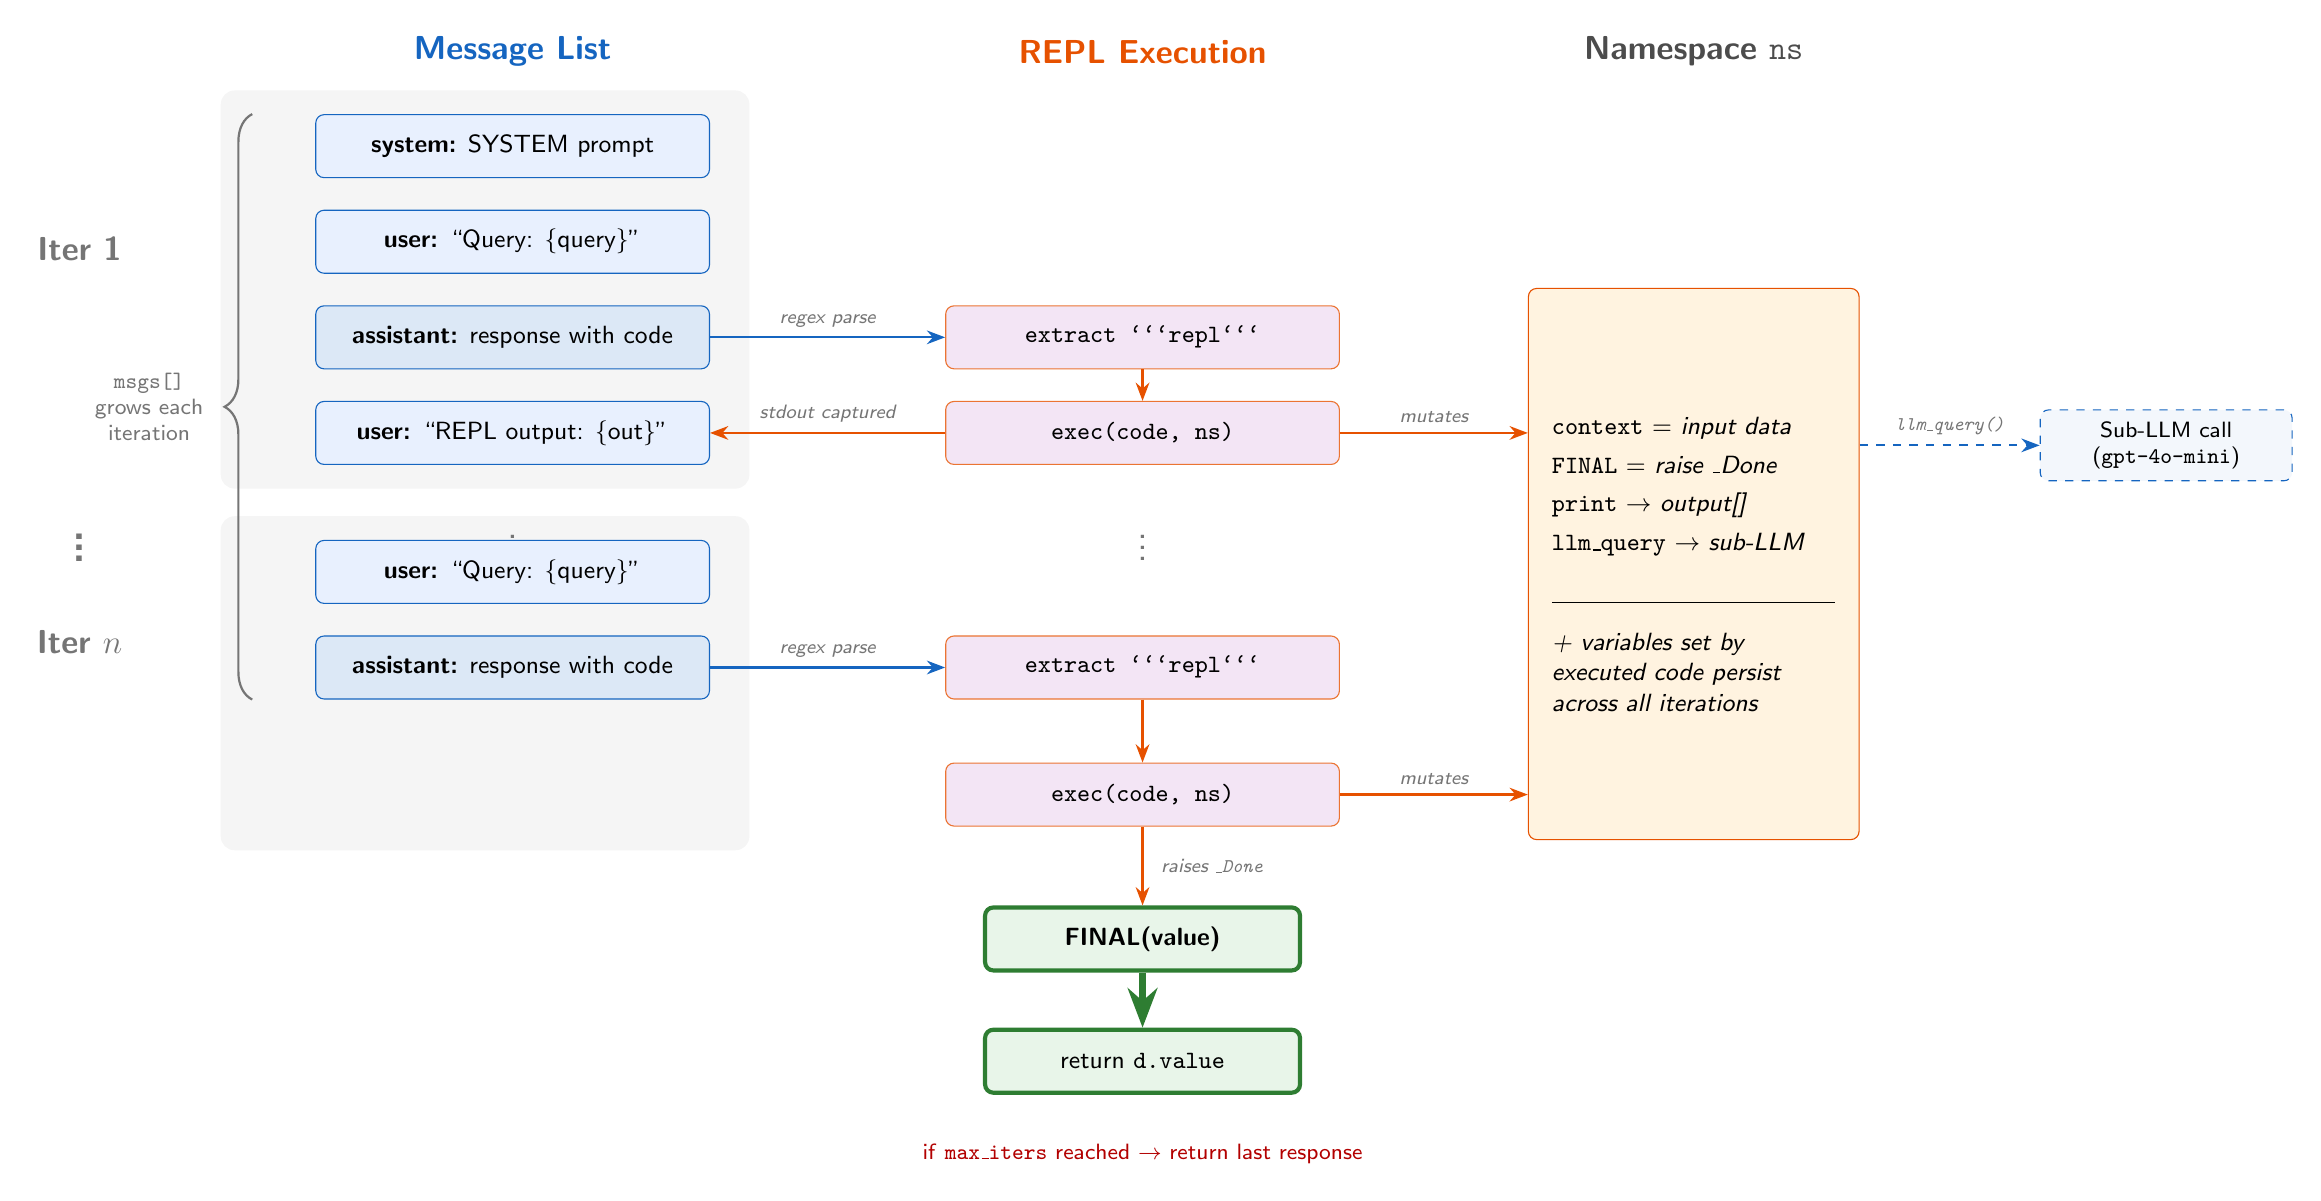
\begin{tikzpicture}[
    >=Stealth,
    font=\sffamily\small,
    msgnode/.style={draw=llmblue, fill=msgbg, rounded corners=3pt,
        minimum width=5cm, minimum height=0.8cm, align=center},
    assistnode/.style={msgnode, fill=llmblue!15},
    nsnode/.style={draw=replorange, fill=nsbg, rounded corners=3pt,
        minimum width=4.2cm, align=left, inner sep=8pt},
    codenode/.style={draw=replorange!80, fill=codebg, rounded corners=3pt,
        minimum width=5cm, minimum height=0.8cm, align=center,
        font=\sffamily\small\ttfamily},
    finalnode/.style={draw=finalgreen, fill=finalbg, rounded corners=3pt,
        minimum width=4cm, minimum height=0.8cm, align=center,
        line width=1.5pt},
    iterlabel/.style={font=\sffamily\bfseries\large, text=graytext},
    ann/.style={font=\sffamily\scriptsize\itshape, text=graytext},
]

% =====================================================
% Column positions
% =====================================================
\def\colmsg{0}
\def\colrepl{8}
\def\colns{15}

% =====================================================
% Column headers
% =====================================================
\node[font=\sffamily\bfseries\large, text=llmblue]
    (hdr-msgs) at (\colmsg, 0) {Message List};
\node[font=\sffamily\bfseries\large, text=replorange]
    (hdr-repl) at (\colrepl, 0) {REPL Execution};
\node[font=\sffamily\bfseries\large, text=black!70]
    (hdr-ns) at (\colns, 0) {Namespace \texttt{ns}};

% =====================================================
% Namespace box (persistent, spans all iterations)
% =====================================================
\node[nsnode, minimum height=7cm, anchor=north] (ns) at (\colns, -3.0) {
    \texttt{context} = \textit{input data}\\[3pt]
    \texttt{FINAL} = \textit{raise \_Done}\\[3pt]
    \texttt{print} $\rightarrow$ \textit{output[]}\\[3pt]
    \texttt{llm\_query} $\rightarrow$ \textit{sub-LLM}\\[8pt]
    \rule{3.6cm}{0.4pt}\\[6pt]
    \textit{+ variables set by}\\
    \textit{executed code persist}\\
    \textit{across all iterations}
};

% =====================================================
% Iteration 1
% =====================================================
\node[iterlabel] (iter1) at (-5.5, -2.5) {Iter 1};

% Messages
\node[msgnode] (sys) at (\colmsg, -1.2) {\textbf{system:} SYSTEM prompt};
\node[msgnode, below=0.4cm of sys] (u1)
    {\textbf{user:} ``Query: \{query\}''};
\node[assistnode, below=0.4cm of u1] (a1)
    {\textbf{assistant:} response with code};

% REPL output feedback message
\node[msgnode, below=0.4cm of a1] (repl1)
    {\textbf{user:} ``REPL output: \{out\}''};

% REPL — Y-aligned with the message nodes they connect to
\node[codenode] (code1) at (\colrepl, 0 |- a1)
    {extract \texttt{```repl```}};
\node[codenode] (exec1) at (\colrepl, 0 |- repl1)
    {\textbf{exec(code, ns)}};

% assistant -> extract (flat horizontal)
\draw[->, thick, llmblue] (a1.east) -- (code1.west)
    node[midway, above, ann] {regex parse};
% extract -> exec
\draw[->, thick, replorange] (code1) -- (exec1);
% exec -> namespace
\draw[->, thick, replorange] (exec1.east) -- (ns.west |- exec1)
    node[midway, above, ann] {mutates};

% exec -> REPL output (flat horizontal back)
\draw[->, thick, replorange] (exec1.west) -- (repl1.east)
    node[midway, above, ann] {stdout captured};

% =====================================================
% Ellipsis between iterations
% =====================================================
\node[font=\sffamily\Huge, text=graytext] at (-5.5, -6.2) {\vdots};
\node[font=\sffamily\Large, text=graytext] at (\colmsg, -6.2) {\vdots};
\node[font=\sffamily\Large, text=graytext] at (\colrepl, -6.2) {\vdots};

% =====================================================
% Iteration N
% =====================================================
\node[iterlabel] (iter2) at (-5.5, -7.5) {Iter $n$};

\node[msgnode, anchor=north] (u2) at (\colmsg, -6.2)
    {\textbf{user:} ``Query: \{query\}''};
\node[assistnode, below=0.4cm of u2] (a2)
    {\textbf{assistant:} response with code};

\node[codenode] (code2) at (\colrepl, 0 |- a2)
    {extract \texttt{```repl```}};
\node[codenode, below=0.8cm of code2] (exec2)
    {\textbf{exec(code, ns)}};

% assistant -> extract (flat horizontal)
\draw[->, thick, llmblue] (a2.east) -- (code2.west)
    node[midway, above, ann] {regex parse};
\draw[->, thick, replorange] (code2) -- (exec2);
\draw[->, thick, replorange] (exec2.east) -- (ns.west |- exec2)
    node[midway, above, ann] {mutates};

% =====================================================
% FINAL exit — generous spacing
% =====================================================
\node[finalnode, below=1.0cm of exec2] (final)
    {\textbf{FINAL(value)}};
\node[finalnode, below=0.7cm of final]
    (ret) {\textsf{return} \texttt{d.value}};

\draw[->, thick, replorange] (exec2.south) -- (final.north)
    node[midway, right=3pt, ann] {raises \texttt{\_Done}};
\draw[->, finalgreen, line width=2.5pt] (final) -- (ret);

% =====================================================
% Sub-LLM callout — lives in namespace, called during exec
% =====================================================
\node[draw=llmblue, dashed, fill=llmblue!5, rounded corners=3pt,
    minimum width=3.2cm, minimum height=0.9cm, align=center,
    font=\sffamily\footnotesize]
    (subllm) at (\colns + 6, -5.0) {Sub-LLM call\\(\texttt{gpt-4o-mini})};

\draw[->, llmblue, dashed, thick]
    (ns.east |- subllm) -- (subllm.west)
    node[midway, above, ann] {\texttt{llm\_query()}};

% =====================================================
% Growing message list brace
% =====================================================
\draw[decorate, decoration={brace, amplitude=10pt, mirror},
    thick, graytext]
    ([xshift=-0.8cm]sys.north west) -- ([xshift=-0.8cm]a2.south west)
    node[midway, left=14pt, align=center,
        font=\sffamily\footnotesize, text=graytext]
    {\texttt{msgs[]}\\grows each\\iteration};

% =====================================================
% Max iters fallback
% =====================================================
\node[font=\sffamily\footnotesize, text=red!70!black, align=center,
    below=0.5cm of ret]
    (maxiter) {if \texttt{max\_iters} reached $\rightarrow$ return last response};

% =====================================================
% Iteration bands (background)
% =====================================================
\begin{pgfonlayer}{background}
    \fill[iterband, rounded corners=5pt]
        ([xshift=-1.2cm, yshift=0.3cm]sys.north west)
        rectangle
        ([xshift=0.5cm, yshift=-0.3cm]repl1.south east |- exec1.south);
    \fill[iterband, rounded corners=5pt]
        ([xshift=-1.2cm, yshift=0.3cm]u2.north west)
        rectangle
        ([xshift=0.5cm, yshift=-0.3cm]a2.south east |- exec2.south);
\end{pgfonlayer}

\end{tikzpicture}
\end{document}
